\section{Experiments}

In this section, we design our experiments to answer the following four research questions:
\begin{itemize}[leftmargin=*,nosep]
    \item \textbf{RQ1:} How does JitRL compare against state-of-the-art training-free baselines and weight-update methods?
    \item \textbf{RQ2:} Does JitRL possess generalization capabilities across unseen tasks and different model backbones?
    \item \textbf{RQ3:}  How does JitRL qualitatively correct the agent's decision-making?
    \item \textbf{RQ4:} How do key components impact JitRL's performance?
\end{itemize}


\begin{table*}[t]
  \caption{Main results on WebArena. We report average (\textbf{Avg}) and final (\textbf{Final}) success rate (\%) for each domain. The gap between Final and Avg reflects learning efficiency. The final column (Average) is calculated as the micro-average across all tasks from all websites.}
  \vskip -0.1in
  \label{tab:main_results}
  \begin{center}
    \begin{small}
      % \begin{sc}
      % \resizebox{\textwidth}{!}{%
        \begin{adjustbox}{width=\textwidth}
        \begin{tabular}{lcccccccccccc}
          \toprule
          \multirow{2}{*}{\textbf{Method}} & \multicolumn{2}{c}{\textbf{Admin}} & \multicolumn{2}{c}{\textbf{GitLab}} & \multicolumn{2}{c}{\textbf{Map}} & \multicolumn{2}{c}{\textbf{Reddit}} & \multicolumn{2}{c}{\textbf{Shopping}} & \multicolumn{2}{c}{\textbf{Average}} \\
          & \textbf{Avg} & \textbf{Final}
          & \textbf{Avg} & \textbf{Final}
          & \textbf{Avg} & \textbf{Final}
          & \textbf{Avg} & \textbf{Final}
          & \textbf{Avg} & \textbf{Final}
          & \textbf{Avg} & \textbf{Final}\\
          \midrule
          Static & 39.46 & 39.67 & 38.92 & 38.24 & 30.62 & 31.25 & 39.60 & 42.86 & 24.06 & 25.00 & 35.63 & 36.30 \\
          Memory & 47.91 & 47.80 & 39.31 & 40.20 & 30.47 & 32.81 & 53.02 & 55.04 & 30.16 & 33.16 & 41.36 & 43.00 \\
          Reflexion & 48.46 & 50.55 & 38.43 & 40.69 & 29.38 & 27.34 & 54.88 & 56.59 & 30.83 & 31.25 & 41.08 & 42.12 \\
          AWM & 49.46 & 51.09 & 37.94 & 40.20 & 34.38 & 32.81 & 55.66 & 58.14 & 23.12 & 22.40 & 39.37 & 40.32 \\
          EvoTest & 44.51 & 47.80 & 37.94 & 39.22 & 33.59 & 41.41 & 51.78 & 54.26 & 26.67 & 29.17 & 39.24 & 42.49 \\
          \midrule
          \textbf{JitRL} & \textbf{52.31} & \textbf{56.59} & \textbf{40.78} & \textbf{45.00} & \textbf{37.66} & \textbf{42.19} & \textbf{57.64} & \textbf{61.98} & \textbf{41.67} & \textbf{45.83} & \textbf{46.98} & \textbf{51.35} \\
          \bottomrule
        \end{tabular}
        \vspace{-6mm}
        \end{adjustbox}
      % }
      % \end{sc}
    \end{small}
  \end{center}
\end{table*}



% \begin{table*}[t]
%   \caption{Main results on WebArena. We report the \textbf{Final} success rate(\%) for each domain.}
%   \vskip -0.1in
%   \label{tab:main_results}
%   \begin{center}
%     \begin{small}
%         \begin{adjustbox}{width=\textwidth}
%         \begin{tabular}{lcccccc}
%           \toprule
%           \textbf{Method} & \textbf{Admin} & \textbf{GitLab} & \textbf{Map} & \textbf{Reddit} & \textbf{Shopping} & \textbf{Average} \\
%           \midrule
%           Static    & 39.67 & 38.24 & 31.25 & 42.86 & 25.00 & 36.30 \\
%           Memory    & 47.80 & 40.20 & 32.81 & 55.04 & 33.16 & 43.00 \\
%           Reflexion & 50.55 & 40.69 & 27.34 & 56.59 & 31.25 & 42.12 \\
%           AWM       & 51.09 & 40.20 & 32.81 & 58.14 & 22.40 & 40.32 \\
%           EvoTest   & 47.80 & 39.22 & 41.41 & 54.26 & 29.17 & 42.49 \\
%           \midrule
%           \textbf{JitRL} & \textbf{56.59} & \textbf{45.00} & \textbf{42.19} & \textbf{61.98} & \textbf{45.83} & \textbf{51.35} \\
%           \bottomrule
%         \end{tabular}
%         \end{adjustbox}
%     \end{small}
%   \end{center}
% \end{table*}



% \begin{table*}[h]
%     \centering
%     \caption{Comparison of \textbf{Final Score} with weight-update methods on WebArena-Lite, the held-out test set used by SFT and WebRL (which train on the remaining WebArena tasks). Despite being training-free, JitRL outperforms online RL fine-tuning without any gradient updates.}
%     \label{tab:webrl_comparison}
%     \begin{tabular}{lcccccc}
%     \toprule
%     \textbf{Method} & \textbf{Admin} & \textbf{GitLab} & \textbf{Map} & \textbf{Reddit} & \textbf{Shopping} & \textbf{Avg} \\
%     \midrule
%     %Llama-3.1-Instruct-70B & 17.1 & 16.7 & 20.0 & 10.5 & 4.4 & 12.7 \\
%     SFT & 20.0 & 20.0 & 26.7 & 52.6 & 13.3 & 23.0 \\
%     WebRL & 54.3 & 50.0 & 40.0 & 78.9 & 44.4 & 49.1 \\
%     %Llama-3.1 + JitRL & 18.33 & 25.29 & 24.67 & 38.00 & 24.00 & 26.06 \\
%     \midrule
%     %Gemini-2.5-Flash & 48.57 & 40.00 & 25.00 & 60.00 & 41.30 & 42.98 \\
%     JitRL & \textbf{65.71} & \textbf{56.67} & \textbf{53.57} & \textbf{78.95} & \textbf{53.33} & \textbf{60.0} \\
%     \bottomrule
%     \end{tabular}
% \end{table*}

\begin{table}[t]
  \caption{
 Comparison of \textbf{Final} success rate (\%) with weight-update methods on \textbf{WebArena-Lite}, the held-out test set. The remainder of WebArena was used to train WebRL.
  }

  \label{tab:webrl_comparison}
  \begin{center}
    \begin{small}
      \begin{adjustbox}{width=\columnwidth}
      \begin{tabular}{lcccccc}
        \toprule
        \textbf{Method} & \textbf{Admin} & \textbf{GitLab} & \textbf{Map} & \textbf{Reddit} & \textbf{Shopping} & \textbf{Average} \\
        \midrule
       SFT    & 20.00 & 20.00 & 26.70 & 52.60 & 13.30 & 23.00 \\
        WebRL & 58.33 & 47.06 & 32.26 & 62.50 & 30.43 & 46.06 \\
        \textbf{JitRL} & \textbf{65.71} & \textbf{56.67} & \textbf{53.57} & \textbf{78.95} & \textbf{53.33} & \textbf{60.00} \\
        \bottomrule
      \end{tabular}
      \vspace{-8mm}
      \end{adjustbox}
    \end{small}
  \end{center}

\end{table}



\begin{table}[ht]
\vspace{-4mm}
    \caption{Results on Jericho games. We report: \textbf{Avg}: average score across 50 episodes; \textbf{Final}: final episode score.}
    \label{tab:jericho_results}
    \begin{center}
    \begin{small}
    % \begin{adjustbox}{width=\columnwidth}
    \begin{tabular}{lcccccc}
    \toprule
    \multirow{2}{*}{\textbf{Method}} & \multicolumn{2}{c}{\textbf{Library}} & \multicolumn{2}{c}{\textbf{Zork1}} & \multicolumn{2}{c}{\textbf{Zork3}} \\
    \cmidrule(lr){2-3} \cmidrule(lr){4-5} \cmidrule(lr){6-7}
    & \textbf{Avg} & \textbf{Final} & \textbf{Avg} & \textbf{Final} & \textbf{Avg} & \textbf{Final} \\
    \midrule
    Static & 10.0 & 10 & 8.5 & 10 & 0.2 & 0 \\
    Memory & 13.2 & 14 & 22.9 & 25 & 1.0 & 1 \\
    Reflexion & 15.4 & 18 & 26.1 & 35 & 1.4 & 1 \\
    AWM & 12.7 & 10 & 38.8 & 44 & 1.9 & 2 \\
    EvoTest & 21.5 & 26 & 46.8 & 54 & 2.6 & 4 \\
    \midrule
    GRPO & 13.6 & 11 & 16.2 & 10 & 1.1 & 2 \\
    
    \midrule
    \textbf{JitRL} & \textbf{25.9} & \textbf{30} & \textbf{53.0} & \textbf{69} & \textbf{3.1} & \textbf{5} \\
    \bottomrule
    \end{tabular}
    \vspace{-4mm}
    % \end{adjustbox}
    \end{small}
    \end{center}
\end{table}

\subsection{Experimental Setup}

\paragraph{Benchmarks.}
We evaluate our method in two distinct environments to demonstrate versatility:



\begin{itemize}[leftmargin=*,nosep]
    \item \textbf{WebArena} \citep{webarena}: A realistic web environment comprising multiple functional websites.
    %, including e-commerce platforms (OneStopShop), code repositories (GitLab), social forums (Reddit), content management systems (CMS), maps, and encyclopedias. 
    It challenges agents to navigate complex DOM trees and execute sequential actions to fulfill user instructions.
    \item \textbf{Jericho} \citep{jericho}: A benchmark suite for interactive fiction games where agents interact purely via textual commands. 
    %This environment rigorously tests the agent's language understanding and ability to optimize strategies across long horizons. 
    We evaluate performance on three representative games: Library, Zork 1, and Zork 3.
\end{itemize}
\paragraph{Baselines.}
We compare JitRL against a comprehensive set of methods, which fall into two paradigms: training-free and weight-update. 

\begin{itemize}[leftmargin=*,nosep]
    \item \textbf{Training-Free Methods.} We evaluate five inference-time strategies:
    (1) \textbf{Static}: A non-learning agent with fixed configuration.
    (2) \textbf{Memory}: An in-context learning baseline that fills the context window with full transcripts of past episodes, utilizing a First-In-First-Out (FIFO) strategy to handle token limits.
    (3) \textbf{Reflexion} \citep{reflexion}: A prompt-based method where the agent generates structured textual self-reflections after each episode to guide subsequent attempts.
    (4) \textbf{AWM} \citep{awm}: An episodic memory approach that extracts and persistently stores reusable workflows derived from successful trajectories.
    (5) \textbf{EvoTest} \citep{evotest}: An evolutionary optimization framework that iteratively rewrites prompts, updates memory with state-action pairs, and dynamically tunes hyperparameters. For JitRL and training-free baselines, we use \texttt{Gemini-2.5-flash} as LLM backbones.

    \item \textbf{Weight-Update Methods}. We compare against leading training approaches. For WebArena, we directly utilize the pre-trained checkpoints for \textbf{SFT} and \textbf{WebRL} provided by \cite{webrl}, both built on \texttt{Llama-3.1-70B-Instruct}. For Jericho, we employ the task-specific \texttt{Qwen3-32B} checkpoints, which are trained via \textbf{GRPO}~\citep{grpo} for each individual game. Refer to Appendix~\ref{app:baselines} for a detailed description of the training process.
\end{itemize}

% \paragraph{Backbone Models.}
% For all gradient-free methods (including JitRL), we utilize Gemini-2.5-Flash as the backbone to ensure a fair comparison on efficient inference. For weight-update baselines (SFT and WebRL), we adopt Llama-3.1-70B-Instruct, following their original configurations.

% \paragraph{Evaluation Metrics.}
% We conduct our evaluation on a task set $\mathcal{T}$, where each task is executed for $L$ consecutive episodes. Let $y_{i,j}$ denote the score for the $i$-th task at the $j$-th episode. For WebArena, $y_{i,j} \in \{0, 1\}$ represents binary task completion (success=1, failure=0); for Jericho, $y_{i,j}$ is the game score. We report two aggregated metrics: (1) \textbf{Average Score (Avg)}: Computed as $\frac{1}{|\mathcal{T}| \cdot L} \sum_{i=1}^{|\mathcal{T}|} \sum_{j=1}^{L} y_{i,j}$, this metric averages scores across all attempts to reflect overall learning efficiency; and (2) \textbf{Final Score (Final)}: Compute as $\frac{1}{|\mathcal{T}|} \sum_{i=1}^{|\mathcal{T}|} y_{i,L}$, this measures the average score of the final episode across all tasks, indicating converged performance. Notably, a larger differential between Final and Avg indicates greater learning gain.


\paragraph{Implementation Details.}
We implement two variants to derive logits for the logit-based policy update. This design specifically addresses the constraint that many black-box models do not expose access to raw log-probabilities:
\begin{itemize}[leftmargin=*,nosep]
    \item \textbf{Token-level Logit}: 
    We prompt the generator to select an action from $k$ candidates by outputting a corresponding index token (e.g., ``1'', ``2''). We then extract the log-probabilities of these tokens as logits.

    \item \textbf{Verbalized Logit}: 
    For models that do not expose log-probabilities, we prompt the LLM to explicitly output a confidence score (0--100) and transform them to logits for each candidate action.
\end{itemize}




More implementation details, such as state representation, memory retrieval, and action handling, can be found in Appendix~\ref{app:implementation}. Prompt templates can be found in Appendix ~\ref{app:prompts}, hyperparameters can be found in Appendix ~\ref{app:hyperparameters}. 


\subsection{RQ1: Main Performance Comparison}
To address RQ1, we employ a multi-trial sequential testing protocol. Instead of evaluating each task only once, the agent executes $L$ consecutive episodes for each task $i$. This setup is designed to simulate a realistic deployment scenario where an agent must improve its performance on-the-fly through repeated interactions. 

%Specifically, this protocol allows us to verify whether JitRL can effectively utilize the cross-episode memory accumulated from earlier attempts (e.g., learning from a failure in episode 1) to refine its policy in subsequent trials (e.g., succeeding in episode 5).


\subsubsection{Results on WebArena}

\paragraph{Metrics.} Our evaluation dataset contains $\mathcal{T}$ tasks, which we run sequentially, each for $L=5$ times, and evaluate performance primarily using the Success Rate. Let $y_{i,j} \in \{0,1\}$ denote the binary completion status (success=1, failure=0) of task $i$ at episode $j$. We report two aggregated metrics: (1) \textbf{Average Success Rate (Avg)}, calculated as $\frac{1}{\mathcal{T}\cdot 5}\sum_{i=1}^{\mathcal{T}}\sum_{j=1}^{5}y_{i,j}$, which averages performance across all attempts to reflect the overall learning efficiency; and (2) \textbf{Final Success Rate (Final)}, computed as $\frac{1}{\mathcal{T}}\sum_{i=1}^{\mathcal{T}}y_{i,5}$, which measures the success rate of the final episode to indicate the agent's converged capability.  Notably, a larger differential between Final and Avg indicates a steeper learning curve, demonstrating that the agent successfully leverages historical memory to improve its policy over time.


Table~\ref{tab:main_results} presents the performance comparison of JitRL and training-free baselines on WebArena. JitRL outperforms all training-free baselines in both cumulative (Avg) and converged (Final) success rates. Moreover, the significant gap between the Avg and Final highlights JitRL's robust learning capability. Performance gains are most pronounced in structured domains like Shopping (+73.2\% over Static) due to high trajectory reusability. In contrast, Reflexion occasionally suffers from ``reflection noise'' in sites like Map, where misleading feedback degrades performance.


Table~\ref{tab:webrl_comparison} compares JitRL with weight-update methods (WebRL) on the held-out WebArena-Lite \citep{webrl} subset, as the remaining WebArena tasks were utilized for training WebRL and SFT. JitRL attains SOTA performance purely through inference-time optimization. This demonstrates that JitRL serves as a highly efficient alternative to computationally intensive training methods. We also provide results with the same backbone in an on-the-fly setting (Appendix~\ref{app:fair_comparison}), and with the same backbone following separate training and evaluation phases (Appendix~\ref{app:large_budget}).




\subsubsection{Results on Jericho}

% \begin{figure*}[htbp]
%     \centering
%     \begin{minipage}[b]{0.32\textwidth}
%         \centering
%         \includegraphics[width=\textwidth]{figures/library.pdf}
%         \centerline{(a) Library}
%     \end{minipage}
%     \hfill
%     \begin{minipage}[b]{0.32\textwidth}
%         \centering
%         \includegraphics[width=\textwidth]{figures/zork1.pdf}
%         \centerline{(b) Zork1}
%     \end{minipage}
%     \hfill
%     \begin{minipage}[b]{0.32\textwidth}
%         \centering
%         \includegraphics[width=\textwidth]{figures/zork3.pdf}
%         \centerline{(c) Zork3}
%     \end{minipage}
%     \caption{Learning curves on Jericho games. JitRL shows consistent improvement across episodes.}
%     \label{fig:jericho}
%     \vskip -0.1in
% \end{figure*}

\begin{figure*}[h]
    \centering
    %\vspace{-4mm}
    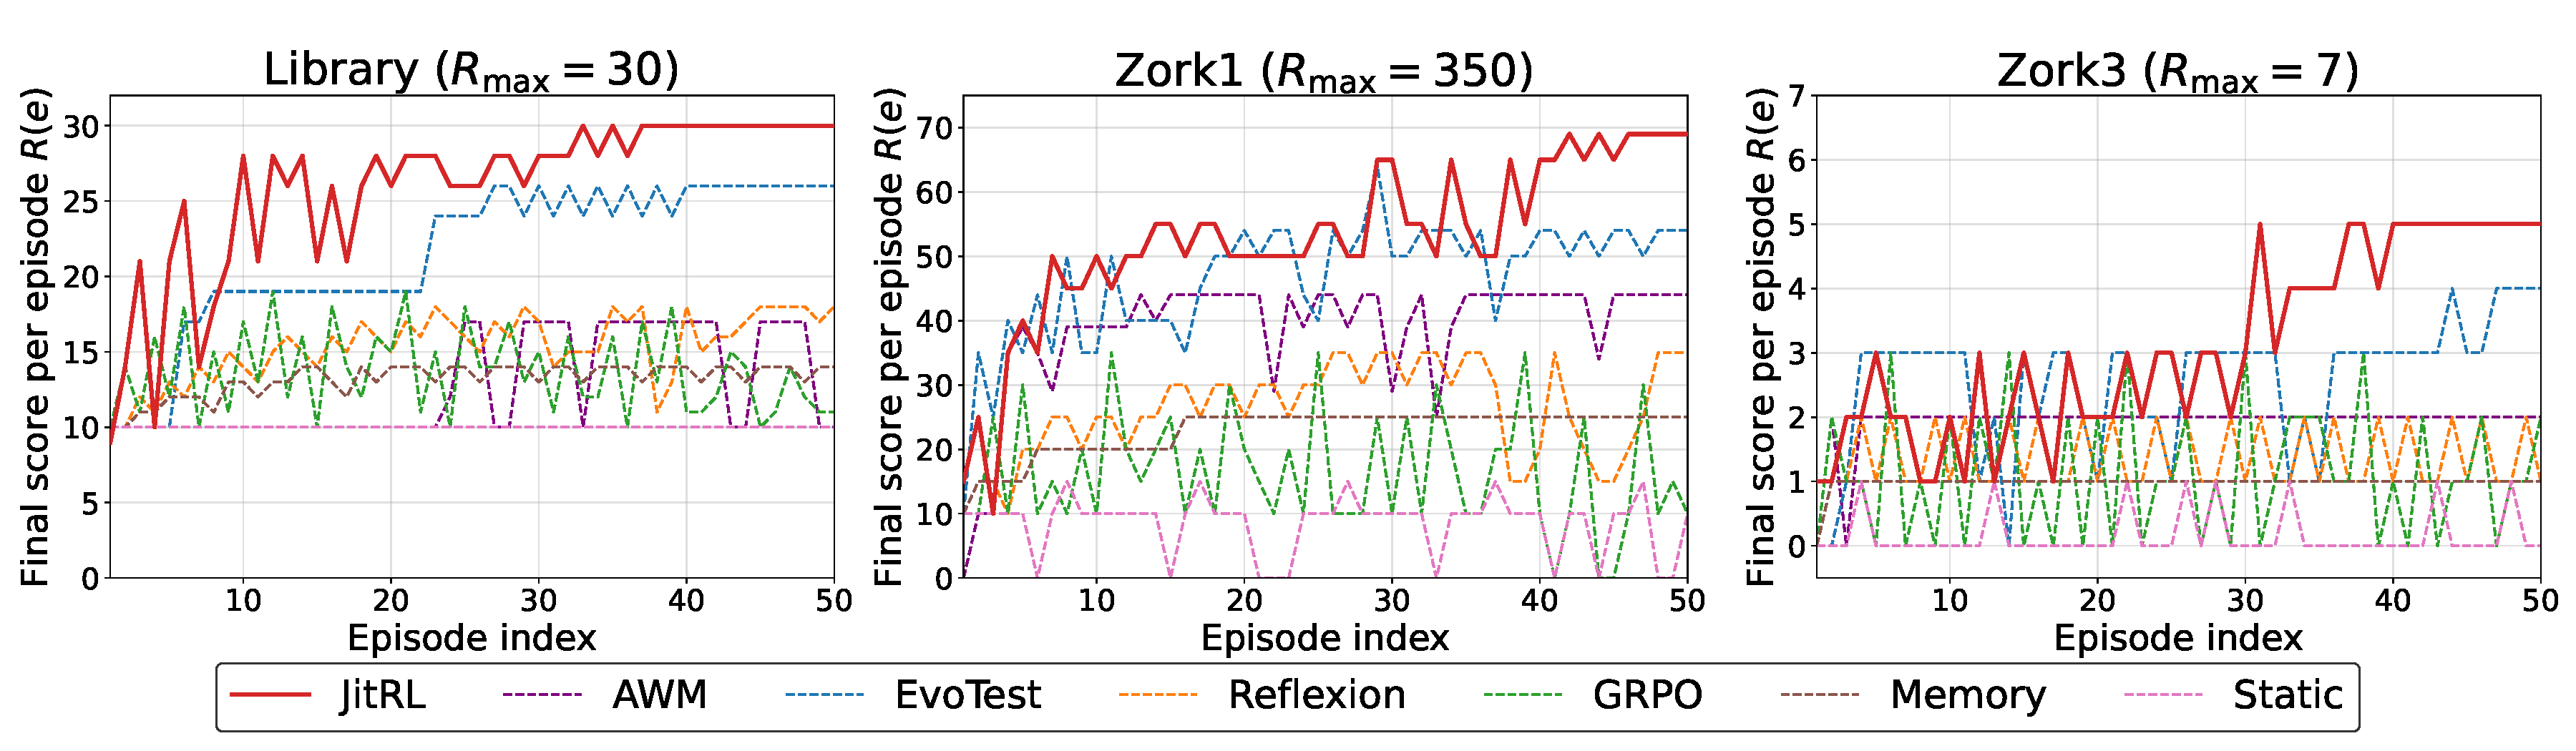
\includegraphics[width=\textwidth]{figures/all_games_performance.pdf}

    \caption{Learning curves on Jericho games. JitRL shows consistent improvement across episodes.}
     \label{fig:jericho}
\end{figure*}


\paragraph{Metrics.} For Jericho, we evaluate the \textbf{Game Score}. Let $y_{i,j}$ represent the score obtained in game $i$ during episode $j$. Similar to WebArena, we report the \textbf{Average Score (Avg)} over 50 episodes to capture the learning stability, and the \textbf{Final Score (Final)} to assess the performance at the final episode.

% Table~\ref{tab:jericho_results} presents the quantitative comparison on Jericho text-based games. JitRL achieves the highest scores across all three games, significantly outperforming all baselines. The substantial gap between Avg and Final scores across all games highlights JitRL's superior learning efficiency---the agent consistently improves over episodes rather than plateauing early.

% Figure~\ref{fig:jericho} depicts the learning curves across the evaluated environments. The results reveal several key insights: (1) JitRL exhibits rapid initial learning, achieving competitive performance within the first 10-15 episodes; (2) the performance gap between JitRL and baselines widens as episodes progress, indicating effective experience accumulation; and (3) JitRL shows reduced variance in later stages, implying stable policy convergence. In contrast, GRPO exhibits high variance throughout, suggesting that gradient-based updates struggle with the sparse reward signals in text-based games. Memory-based approaches (Memory, AWM) plateau early, this is because they over-rely on established memory patterns, which inhibit further exploration and cause the agents to converge prematurely to suboptimal policies.



Table~\ref{tab:jericho_results} presents the quantitative comparison on Jericho. JitRL achieves the highest scores across all three games, significantly outperforming baselines. The learning curves for each episode are visualized in Figure~\ref{fig:jericho}, which reveal several key insights: (1) \textbf{JitRL exhibits rapid initial learning}, achieving competitive performance within the first 10-15 episodes; (2) \textbf{the performance gap between JitRL and baselines widens as episodes progress}, indicating effective experience accumulation; and (3) \textbf{JitRL shows reduced variance in later stages}, implying stable policy convergence. In contrast, GRPO exhibits high variance throughout, suggesting that gradient-based updates struggle with the sparse reward signals. Memory-based approaches (Memory, AWM) plateau early, because they over-rely on established memory patterns, which inhibit further exploration and cause the agents to converge to suboptimal policies. A same-backbone comparison between JitRL and GRPO is provided in Appendix~\ref{app:same_backbone_jericho}.

\begin{table}[t]
  \caption{Comparison of average (\textbf{Avg}) and \textbf{Final} success rate between JitRL and baseline methods across different backbone LLMs.}
  \vskip 0.1in
  \label{tab:base_models}
  \begin{center}
    \begin{small}
        \begin{tabular}{lcccc}
          \toprule
          \multirow{2}{*}{\textbf{Method}} 
          & \multicolumn{2}{c}{\textbf{Admin}} 
          & \multicolumn{2}{c}{\textbf{Reddit}} \\
          \cmidrule(lr){2-3} \cmidrule(lr){4-5}
          & \textbf{Avg} & \textbf{Final}
          & \textbf{Avg} & \textbf{Final} \\
          
          % Gemini-2.5-flash
          \midrule
          \multicolumn{5}{c}{\textit{\textbf{Gemini-2.5-flash}}} \\ \addlinespace[2pt]
          Static & 39.46 & 39.67 & 39.60 & 42.86 \\
          Memory & 47.91 & 47.80 & 53.02 & 55.04 \\
          Reflexion & 48.46 & 50.55 & 54.88 & 56.59 \\
          AWM & 49.46 & 51.09 & 55.66 & 58.14 \\
          EvoTest & 44.51 & 47.80 & 51.78 & 54.26 \\
          \textbf{JitRL (Ours)} & \textbf{52.31} & \textbf{56.59} & \textbf{57.64} & \textbf{61.98} \\

          % GPT-5-mini
          \midrule
          \multicolumn{5}{c}{\textit{\textbf{GPT-5-mini}}} \\ \addlinespace[2pt]
          Static & 37.07 & 37.50 & 47.29 & 46.51 \\
          Memory & 43.04 & 45.65 & 50.54 & 51.94 \\
          Reflexion & 40.43 & 41.30 & 49.15 & 49.61 \\
          AWM & 40.00 & 40.22 & 50.23 & 51.94 \\
          EvoTest & 42.93 & 43.48 & 51.94 & 53.49 \\
          \textbf{JitRL (Ours)} & \textbf{48.04} & \textbf{51.63} & \textbf{52.87} & \textbf{57.36} \\

          % DeepSeek-V3.2 
          \midrule
          \multicolumn{5}{c}{\textit{\textbf{DeepSeek-V3.2}}} \\ \addlinespace[2pt]
          Static & 32.07 & 32.61 & 42.02 & 43.41 \\
          Memory & 37.07 & 45.65 & 51.47 & 56.28 \\
          Reflexion & 38.04 & 40.22 & \textbf{55.04} & 56.59 \\
          AWM & 42.07 & 44.02 & 52.71 & 55.04 \\
          EvoTest & 44.35 & 45.65 & 50.85 & 53.49 \\
          \textbf{JitRL (Ours)} & \textbf{50.65} & \textbf{54.35} & 54.42 & \textbf{61.24} \\
          \bottomrule
        \end{tabular}
    \end{small}
  \end{center}
  \vskip -0.1in
\vspace{-4mm}
\end{table}



\subsection{RQ2: Generalization Capabilities}

% \begin{table}[htbp]
%     \centering
%     \caption{Zero-Shot Generalization to Unseen Tasks. We report the success rate (\%) where the agent is restricted to retrieving memories exclusively from disjoint tasks.}
%     \label{tab:first_run_comparison}
%     \small
%     \begin{tabular}{lcccccc}
%     \toprule
%     Method & Admin & GitLab & Map & Reddit & Shopping & \textbf{Overall} \\
%     \midrule
%     Static & 36.96 & 37.25 & 31.19 & 36.43 & 23.44 & 33.01 \\
%     Memory & 47.83 & 37.75 & 33.03 & 50.39 & 26.04 & 38.63 \\
%     Reflexion & 46.74 & 34.80 & 31.19 & 48.84 & 31.77 & 38.51 \\
%     AWM & 47.28 & 36.27 & 34.86 & 53.49 & 23.44 & 38.26 \\
%     EvoTest & 43.48 & 35.78 & 34.86 & 49.61 & 18.75 & 35.57 \\
%     \midrule
%     \textbf{JitRL} & \textbf{48.37} & \textbf{38.73} & \textbf{35.78} & \textbf{55.04} & \textbf{36.98} & \textbf{42.67} \\
%     \bottomrule
%     \end{tabular}
% \end{table}


\begin{table}[t]
  \caption{Generalization to Unseen Tasks. We report the average success rate (\%) where the agent is restricted to retrieving memories exclusively from disjoint tasks.}
  \label{tab:first_run_comparison}
  \begin{center}
    \begin{small}
      \begin{adjustbox}{width=\columnwidth}
      \begin{tabular}{lccccc}
        \toprule
        \textbf{Method} & \textbf{Admin} & \textbf{GitLab} & \textbf{Map} & \textbf{Reddit} & \textbf{Shopping} \\
        \midrule
        Static & 36.96 & 37.25 & 31.19 & 36.43 & 23.44 \\
        Memory & 47.83 & 37.75 & 33.03 & 50.39 & 26.04 \\
        Reflexion & 46.74 & 34.80 & 31.19 & 48.84 & 31.77 \\
        AWM & 47.28 & 36.27 & 34.86 & 52.71 & 23.44 \\
        EvoTest & 43.48 & 35.78 & 34.86 & 48.06 & 18.75 \\
        \midrule
        \textbf{JitRL} & \textbf{48.37} & \textbf{38.73} & \textbf{35.78} & \textbf{55.04} & \textbf{36.98} \\
        \bottomrule
      \end{tabular}
      \end{adjustbox}
    \end{small}
  \end{center}
\end{table}



% \begin{figure}
%     \centering
%     \includegraphics[width=1\linewidth]{figures/overlapped_comparison.pdf}
%     \caption{Generalization to Unseen Tasks. We report the average success rate (\%) where the agent is restricted to retrieving memories exclusively from disjoint tasks.}
%     \label{fig:cross_task}
%    \vspace{-2mm}
% \end{figure}
% \begin{table}[t]
% \centering
% \caption{Memory utilization breakdown by domain. Cross-Task refers to memories retrieved from different tasks, while Cross-Episode refers to memories from prior episodes of the same task.}
% \label{tab:memory_utilization}
% \resizebox{0.48\textwidth}{!}{
% \begin{tabular}{lcc}
% \toprule
% \textbf{Domain} & \textbf{Cross-Task (\%)} & \textbf{Cross-Episode (\%)} \\
% \midrule
% Shopping & 62.19 & 37.81 \\
% Admin & 40.54 & 59.46 \\
% Map & 37.64 & 62.36 \\
% \midrule
% \textbf{Average} & \textbf{50.54} & \textbf{49.46} \\
% \bottomrule
% \end{tabular}
% }
% \end{table}


\begin{table}[t]
\vspace{-4mm}
  \caption{Distribution (\%) of cross-task memory utilization.}
  \label{tab:memory_utilization}
  \begin{center}
    \begin{small}
      \begin{adjustbox}{width=\columnwidth}
      \vspace{-6mm}
        \begin{tabular}{lccccc}
          \toprule
          \textbf{Admin} & \textbf{GitLab} & \textbf{Map} & \textbf{Reddit} & \textbf{Shopping} & \textbf{Avg} \\
          \midrule
          40.54 & 38.47 & 37.64 & 56.31 & 62.19 & 47.03 \\
          \bottomrule
        \end{tabular}
      \end{adjustbox}
    \end{small}
  \end{center}
  \vspace{-4mm}
\end{table}


\begin{table*}[t]
    \centering
    \caption{\textbf{Qualitative Analysis of Policy Improvement.} We select three representative cases showing how JitRL modifies decision-making. \textbf{Base} and \textbf{JitRL} denote the logits before and after the memory-based update. Compared to \textbf{Base}, \textbf{JitRL} decreases the logits for \textcolor{red}{\textbf{incorrect}} options and increases them for \textcolor{green!60!black}{\textbf{correct}} options. In this way, JitRL corrects semantic priors and optimizes efficiency.}
    \label{tab:case_study}
    \vspace{8pt}
    \small
    \renewcommand{\arraystretch}{1.2} % 保持增加的行高，视觉舒适
    
    % 确保导言区有 \usepackage{multirow} 和 \usepackage{tabularx}
    \begin{tabularx}{\linewidth}{l l c c >{\raggedright\arraybackslash}X}
        \toprule
        \textbf{Task} & \textbf{Candidate Action} & \textbf{Base} & \textbf{JitRL} & \textbf{Mechanism Explanation} \\
        \midrule
        
        % Case 1: Admin

        Find customer reviews & \textcolor{red}{\textbf{click(CATALOG)}} & \textbf{0.90} & 0.40 & \multirow{2}{=}{While ``Catalog'' appears semantically intuitive, memory corrects this prior: reviews are located under ``Marketing''.} \\
        (Site Functionality) & \textcolor{green!60!black}{\textbf{click(MARKETING)}} & 0.70 & \textbf{1.40} &  \\ 

        \addlinespace[3pt]

        % Case 2: Reddit
        Find posts in subreddit  & \textcolor{red}{\textbf{fill(Search, ``..'')}} & \textbf{0.95} & 0.45 & \multirow{2}{=}{Global search often yields noisy results. Memory steers the agent toward ``Forums'' for a deterministic and accurate path.} \\
        (Navigation Precision) & \textcolor{green!60!black}{\textbf{click(Forums)}} & 0.80 & \textbf{1.80} &  \\

        \addlinespace[3pt]

        % Case 3: Shopping
        Access product inventory & \textcolor{red}{\textbf{click(Products)}} & \textbf{0.95} & -0.28 & \multirow{2}{=}{Clicking loads a generic page. Memory identifies ``hover'' as an efficient shortcut to instantly reveal subcategories.} \\
        (UI Mechanics) & \textcolor{green!60!black}{\textbf{hover(Products)}} & 0.40 & \textbf{0.90} &  \\
        
        \bottomrule

    \end{tabularx}
\end{table*}


        % \addlinespace[6pt]

        % % Case 4: Map - Measure walking distance
        % Measure walking distance & \textcolor{red}{\textbf{fill(Search, "...")}} & \textbf{0.95} & 0.78 & Searching location first is intuitive but inefficient. JitRL \\
        % (Map) & \textcolor{green!60!black}{\textbf{click(Find directions)}} & 0.90 & \textbf{1.40} & learns to directly click ``Find directions'' for distance queries. \\

        % \addlinespace[6pt]

        % % Case 5: Shopping - Browse product category
        % Browse Cabinets category & \textcolor{red}{\textbf{hover(Office Products)}} & \textbf{0.85} & 0.98 & ``Cabinets'' seems related to office furniture, but memory \\
        % (Shopping) & \textcolor{green!60!black}{\textbf{hover(Home \& Kitchen)}} & 0.80 & \textbf{1.80} & knows this category is actually under ``Home \& Kitchen''. \\
To answer RQ2, we assess the universality of our framework. This section evaluates JitRL's performance across different LLM backbones and investigates its zero-shot generalization on unseen tasks where no direct historical memory exists.

\paragraph{Generalization Across Backbones.}
We further evaluate JitRL on GPT-5-mini and DeepSeek-V3.2 \citep{deepseek} to assess its generalizability against other baselines. As shown in Table~\ref{tab:base_models}, JitRL achieves state-of-the-art performance in most cases. This indicates that our logit-update mechanism is model-agnostic and robustly enhances the capabilities of efficient models without parameter tuning.

\paragraph{Cross Task Generalization.}
We assess cross-task generalization on WebArena by simulating a cold-start setting, where the agent utilizes memories solely from disjoint tasks.
As shown in Table~\ref{tab:first_run_comparison}, JitRL consistently outperforms baselines, indicating effective transfer of abstract procedural knowledge rather than specific solutions.



\subsection{Qualitative Analysis: Correcting Semantic Priors}

\label{sec:case_study}

To provide an intuitive understanding of JitRL's mechanism, we examine representative cases where the retrieved memory successfully overrides the base model's erroneous intuition. As shown in Table~\ref{tab:case_study}, regarding \textbf{Site Functionality}, the agent learns to ignore intuitive but incorrect links (e.g., Catalog'') and instead navigates to the correct section (Marketing''). Similarly, for \textbf{Navigation Precision}, memory steers the agent away from noisy global searches toward deterministic navigation links. Additionally, in terms of \textbf{UI Mechanics}, JitRL optimizes interaction efficiency, identifying shortcuts such as prioritizing hover actions to directly reveal fine-grained subcategories rather than clicking into broad category pages.
Additional case studies on Jericho can be found in Appendix~\ref{app:case_jericho}.


\subsection{Qualitative Analysis: Importance of Cross-Task Memory}
We observe the retrieval patterns when both cross-task memory and cross-episode memory are enabled. As shown in Table~\ref {tab:memory_utilization}, cross-task memory accounts for nearly 50\% of the retrieved context, indicating a substantial reliance on this mechanism alongside cross-episode memory. Furthermore,  websites that trigger a higher frequency of cross-task memory retrieval also demonstrate superior cross-task generalization performance compared to Static. 
% \subsubsection{Mechanism Analysis}

% We investigate the underlying mechanisms by answering two questions: is direct logit update superior to prompting, and does the model rely on rote memorization or transferable procedural knowledge?



% \paragraph{Memory Utilization}
% % \begin{table}[t]
% \centering
% \caption{Memory utilization breakdown by domain. Cross-Task refers to memories retrieved from different tasks, while Cross-Episode refers to memories from prior episodes of the same task.}
% \label{tab:memory_utilization}
% \resizebox{0.48\textwidth}{!}{
% \begin{tabular}{lcc}
% \toprule
% \textbf{Domain} & \textbf{Cross-Task (\%)} & \textbf{Cross-Episode (\%)} \\
% \midrule
% Shopping & 62.19 & 37.81 \\
% Admin & 40.54 & 59.46 \\
% Map & 37.64 & 62.36 \\
% \midrule
% \textbf{Average} & \textbf{50.54} & \textbf{49.46} \\
% \bottomrule
% \end{tabular}
% }
% \end{table}


\begin{table}[t]
\vspace{-4mm}
  \caption{Distribution (\%) of cross-task memory utilization.}
  \label{tab:memory_utilization}
  \begin{center}
    \begin{small}
      \begin{adjustbox}{width=\columnwidth}
      \vspace{-6mm}
        \begin{tabular}{lccccc}
          \toprule
          \textbf{Admin} & \textbf{GitLab} & \textbf{Map} & \textbf{Reddit} & \textbf{Shopping} & \textbf{Avg} \\
          \midrule
          40.54 & 38.47 & 37.64 & 56.31 & 62.19 & 47.03 \\
          \bottomrule
        \end{tabular}
      \end{adjustbox}
    \end{small}
  \end{center}
  \vspace{-4mm}
\end{table}


% To investigate whether JitRL relies on rote memorization or effective knowledge transfer, we analyze the composition of retrieved memories. As shown in Table~\ref{tab:memory_utilization}, approximately half of the retrieved memories originate from different tasks (cross-task). This substantial proportion indicates that the agent captures abstract procedural knowledge rather than specific solutions. For instance, an agent querying “price range of mouth guards” retrieves memories from “price range of wireless earphones,”  allowing the agent to reuse successful logical structures despite varying entities. Consequently, this cross-task memory serves as a structural prior, effectively alleviating the cold-start problem by transferring procedural capabilities to semantically related but unseen tasks.

% We analyze memory composition in Table~\ref{tab:memory_utilization}. Approximately half of the retrievals are \textbf{cross-task}, demonstrating substantial knowledge transfer. This is most pronounced in \textbf{Shopping} (62.19\%), where search workflows generalize across different items (e.g., ``mouth guards'' vs. ``earphones''). Similarly, \textbf{Admin} benefits from bootstrapping structurally identical tasks with different parameters. Even in \textbf{Map}, which relies heavily on cross-episode history (62.36\%), cross-task memory still aids in resolving common query patterns. These results confirm that cross-task memory serves as a \textbf{structural prior}, effectively alleviating the cold-start problem by transferring procedural knowledge.


\subsection{RQ4: Ablation Studies}
Finally, we address RQ4 by analyzing the sensitivity of JitRL to key components.
\begin{table}[t]
  %\vspace{-4mm}
  \caption{Ablation: Logit update vs. prompting on WebArena.}
  \label{tab:logit_vs_prompt}
  \begin{center}
    \begin{small}
      \begin{tabular}{lcc}
        \toprule
        \textbf{Method} & \textbf{Admin} & \textbf{Reddit} \\
        \midrule
        JitRL (Prompt Update) & 48.35 & 54.57 \\
        JitRL (Logit Update) & \textbf{52.31} & \textbf{57.64} \\
        \bottomrule
      \end{tabular}
    \end{small}
  \end{center}
  %\vspace{-6mm}
\end{table}

\textbf{Impact of Logit Update.}
To investigate whether the performance gain stems from the logit update mechanism or just the retrieved information, we compare JitRL's \textbf{Logit Update} against \textbf{Prompt Update}, which uses the exact same memory retrieval but appends them to the prompt instead of modifying logits. Table~\ref{tab:logit_vs_prompt} shows that direct Logit Update outperforms Prompt Update on Admin and Reddit websites. We attribute this to the limitations of prompting: as context length grows, LLMs often struggle to attend to retrieved cues or fail to strictly follow instructions. In contrast, our logit update directly modulates the output distribution, ensuring the agent effectively exploits historical advantages.




\begin{figure}[h]
    \centering
    %\vspace{-4mm}
    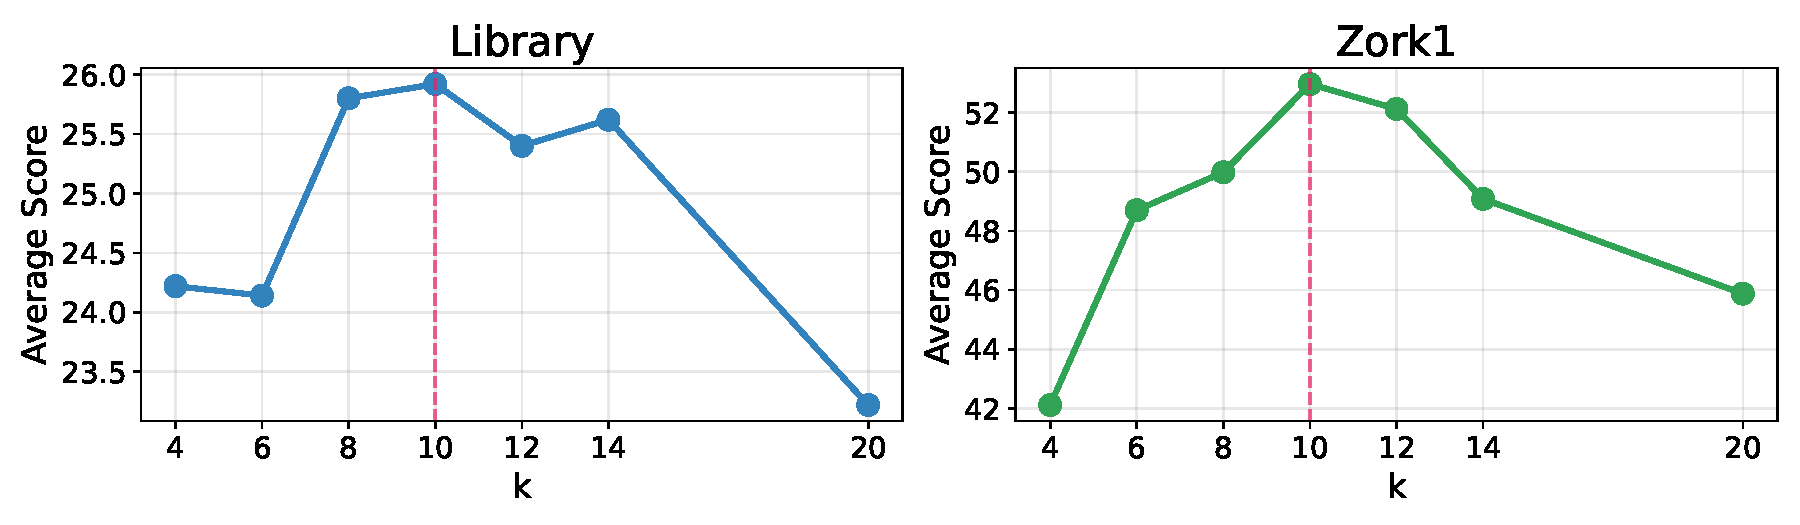
\includegraphics[width=\columnwidth, page=1]{figures/avg_vs_k.pdf}

    \caption{Impact of Retrieval Neighbor Count ($k$).}
    %\vspace{-3mm}
    \label{fig:k}
\end{figure}
% Figure ~\ref{fig:k} illustrates the impact of retrieval neighbor count (k) on agent performance across two text-based game environments. We observe a consistent information-noise trade-off pattern in both Library and Zork1. With k=4, the agent exhibits limited learning capability due to insufficient historical context, resulting in persistent variance and suboptimal final performance (Library: 23.9, Zork1: 48.0 in final 10 episodes). With k=20, early-stage performance suffers from noise introduced by excessive retriev。al, but the agent eventually converges to near-optimal performance as high-quality experiences accumulate (Library: 30.0, Zork1: 60.4). With k=10, the agent achieves the best overall performance, converging to maximum scores in Library (30.0) and reaching the highest final performance in Zork1 (67.8), demonstrating that this configuration strikes an effective balance between retrieving sufficient relevant experiences and avoiding noise contamination. These results suggest that the optimal retrieval count is a critical hyperparameter in memory-augmented agents: too few neighbors provide insufficient context for learning, while too many introduce noise that delays convergence.

% Figure~\ref{fig:k} illustrates the impact of retrieval neighbor count ($k$), revealing a clear information-noise trade-off. A small $k$ limits learning capability due to insufficient historical context, resulting in persistent variance. Conversely, a large $k$ introduces excessive noise that delays convergence in early stages. We find that an intermediate value ($k=10$) strikes the optimal balance, achieving the best performance by securing sufficient relevant experiences while minimizing noise contamination.
\textbf{Impact of Retrieval Neighbor Count.} We evaluate the impact of retrieval neighbor count ($k$) on  Library and Zork1. As shown in Figure~\ref{fig:k}, the agent achieves robust performance with $k$ ranging from 8 to 14. Outside this range, performance degrades due to the trade-off between context sufficiency and noise: a small $k$ limits the historical evidence needed for stable value estimation, leading to high variance, while a large $k$ introduces excessive noise that hinders efficient exploration and delays convergence.

More ablation studies such as the impact of state representation can be found in Appendix ~\ref{app:state_representation}.



% \subsection{Cost Efficiency}
% \input{tables/cost_comparison}
% Table~\ref{tab:cost_comparison} compares the relative API costs across different methods. The results highlight a striking disparity: \textbf{WebRL} incurs prohibitive costs (\$10,000) due to its heavy reliance on online curriculum learning, which necessitates massive trajectory collection and iterative gradient updates. In stark contrast, \textbf{JitRL} (\$98) reduces computational expenses by two orders of magnitude ($\sim$100$\times$). Although JitRL introduces a marginal overhead compared to the Static baseline (\$70) due to memory retrieval, this cost is negligible compared to training-based methods. Consequently, JitRL offers a superior cost-performance ratio, enabling SOTA-level capabilities at a fraction of the deployment cost.

\subsection{Cost Comparison}

We compare the monetary costs of JitRL against all baselines. As shown in Table~\ref{tab:all_baselines_cost}, the weight-update method, WebRL, incurs massive overheads when trained on  \texttt{Llama-3.1-70B-Instruct}. The costs are estimated based on training expenses on NVIDIA H200 GPUs. In contrast, JitRL aligns with other training-free methods whose costs are calculated based on API usage prices. Despite its lower cost, JitRL achieves superior performance, as demonstrated in our main experiments. The detailed cost analysis can be found in Appendix ~\ref{app:cost}.


\begin{table}[ht]
    \centering
    \setlength{\tabcolsep}{1.5pt}
    \caption{Comparison of training cost. }
    \label{tab:all_baselines_cost}
    \resizebox{\linewidth}{!}{
    \begin{tabular}{lccccccc}
        \toprule
        \textbf{Metric} & \textbf{Static} & \textbf{Memory} & \textbf{Reflexion} & \textbf{AWM} & \textbf{EvoTest} & \textbf{WebRL} & \textbf{JitRL} \\
        \midrule
       % \textbf{Time} & 0 & 0 & 0 & 0 & 0 & $\sim$72h & \textbf{0} \\
        \textbf{Cost} & \$200 & \$230 & \$220 & \$250 & \$220 & $\sim$\$9900 & \$290 \\
        \bottomrule
    \end{tabular}
    }
\end{table}
 